\documentclass[a4paper]{article}

\usepackage[english]{babel}
\usepackage[utf8]{inputenc}
\usepackage{amsmath}
\usepackage{graphicx}
\usepackage[colorinlistoftodos]{todonotes}
\usepackage{float}
\usepackage{subfigure}
\usepackage{subfloat}

\title{CS294 Deep RL Assignment 4: Model-Based RL}

\author{Mohamed Khodeir}

\date{\today}

\begin{document}
\maketitle


\section*{Problem 1}
\begin{figure}[H]
\centering
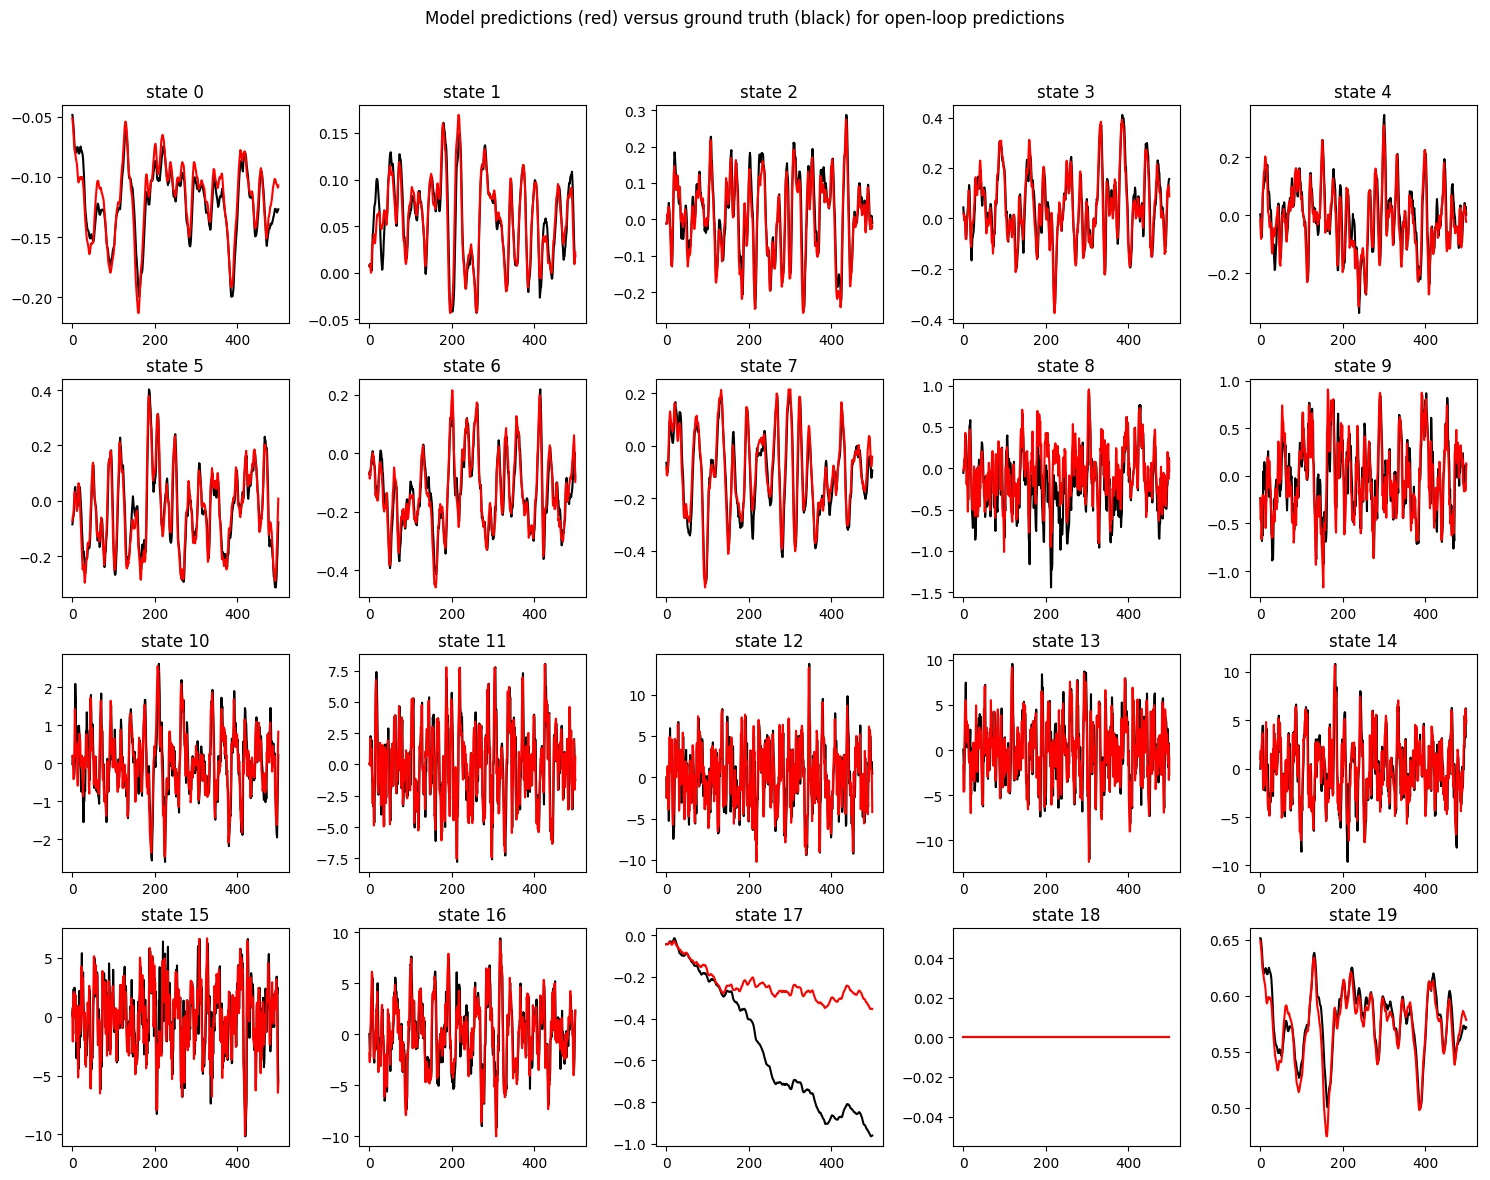
\includegraphics[width=1\textwidth]{p1.jpg}
\caption{State 17 seems to be the most inaccurate. I don't know why. Maybe it's a more complex function?}
\end{figure}

\pagebreak


\section*{Problem 2}
\begin{table}[H]
\begin{tabular}{lllll}
\cline{2-3}
\multicolumn{1}{l|}{}                    & \multicolumn{1}{l|}{\textbf{Random Policy}} & \multicolumn{1}{l|}{\textbf{Trained Policy}} &  &  \\ \cline{1-3}
\multicolumn{1}{|l|}{\textbf{ReturnAvg}} & \multicolumn{1}{l|}{-147.13}                & \multicolumn{1}{l|}{20.9676}                 &  &  \\ \cline{1-3}
\multicolumn{1}{|l|}{\textbf{ReturnStd}} & \multicolumn{1}{l|}{29.8119}                & \multicolumn{1}{l|}{16.1825}                 &  &  \\ \cline{1-3}
                                         &                                             &                                              &  & 
\end{tabular}
\caption{ReturnAvg and ReturnStd for the random policy and for
model-based controller trained on randomly gathered data.}
\end{table}

\pagebreak

\section*{Problem 3a}
\begin{figure}[H]
\centering
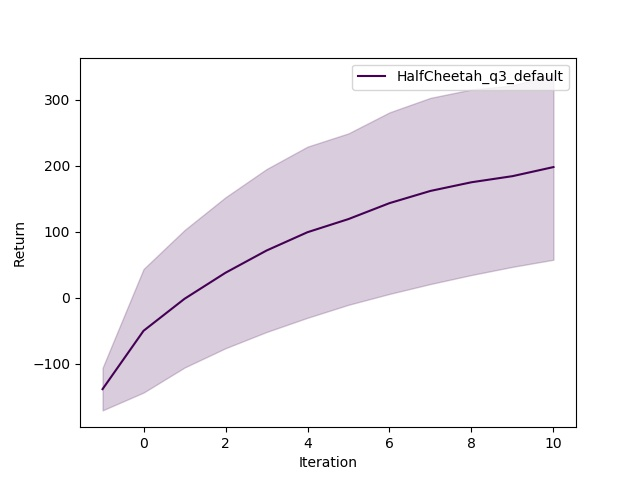
\includegraphics[width=1\textwidth]{p3a.jpg}
\caption{Plot of the returns versus iteration when running model-based reinforcement learning.}
\end{figure}

\pagebreak

\section*{Problem 3b}
\begin{figure}[H]
\centering
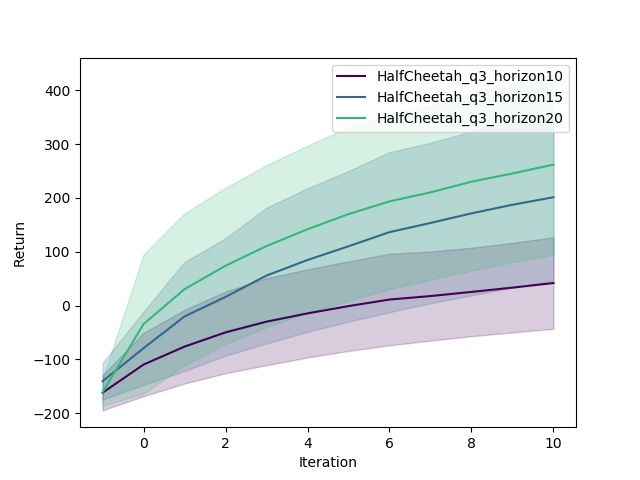
\includegraphics[width=1\textwidth]{p3ba.jpg}
\caption{Plot comparing performance when varying the MPC horizon.}
\end{figure}
\begin{figure}[H]
\centering
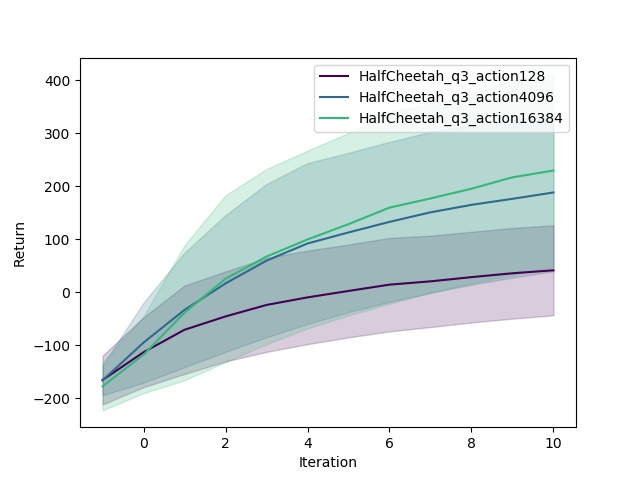
\includegraphics[width=1\textwidth]{p3bb.jpg}
\caption{Plot comparing performance when varying the number of randomly sampled action sequences used for planning.}
\end{figure}
\begin{figure}[H]
\centering
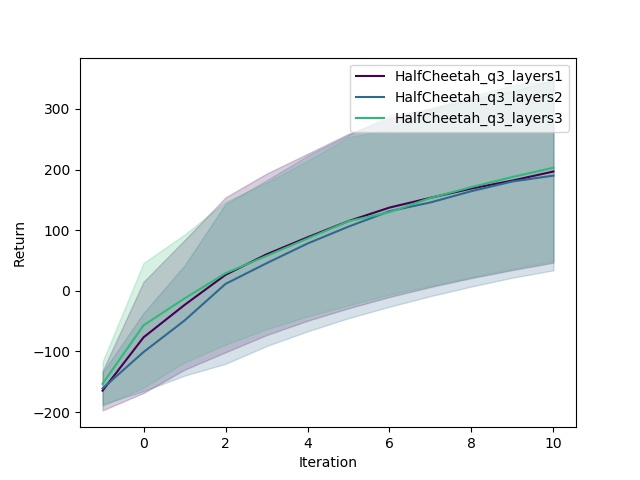
\includegraphics[width=1\textwidth]{p3bc.jpg}
\caption{Plot comparing performance when varying the number of neural network
layers for the learned dynamics model.}
\end{figure}


\end{document}
